\colorformatcornflowerblue

\begin{document}

% -------------------------------------------------------------------------------
% -------------------------------------------------------------------------------

\begin{frame}[plain]
  
\titlepage

\vspace{-1cm}

\begin{center}
\hspace{-4.5cm}
\includegraphics[scale=0.4]{INESCTEC}\\ \vspace{-2.5cm}\hspace{4.5cm}

\includegraphics[scale=0.45]{unine}
\end{center}

\end{frame}

% -------------------------------------------------------------------------------
% -------------------------------------------------------------------------------

\begin{frame}[plain]{}

\begin{snugshade}
  \begin{center}
    Disclaimer: \\Everyone in this room is more knowledgeable \\ about middleware systems than I am.
  \end{center}
\end{snugshade}


\vspace{1cm}

\begin{center}

\includegraphics[scale=0.45]{stupid}  
\end{center}

\end{frame}

% -------------------------------------------------------------------------------

\subtitle[Introduction]{Introduction}

% -------------------------------------------------------------------------------

\begin{frame}{A very simple problem ...}
  
  \begin{itemize}
  \item A set of processes in a network broadcast events, and each process must deliver every event to the application in total order.
  \end{itemize}

\centering


\only<1>
{
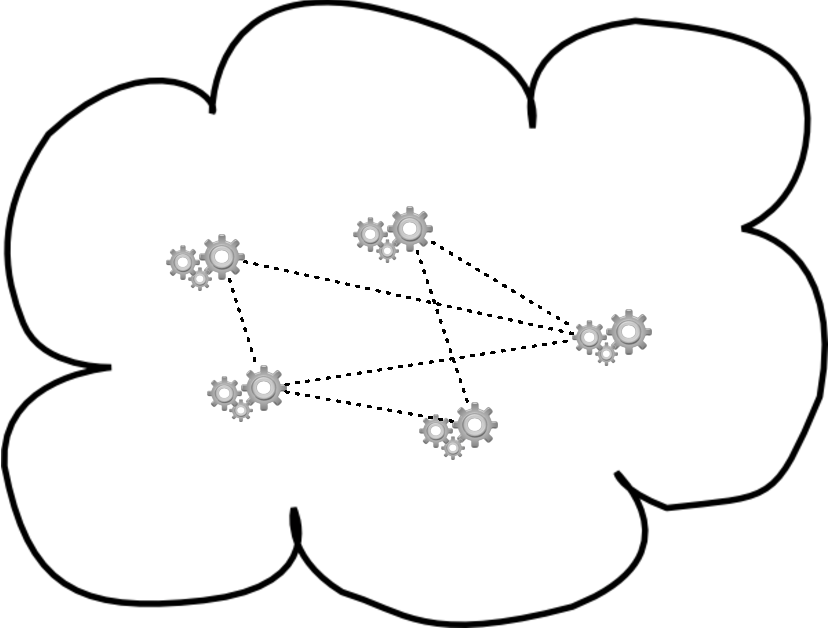
\includegraphics[scale=0.5]{idea}
}

\only<2>
{
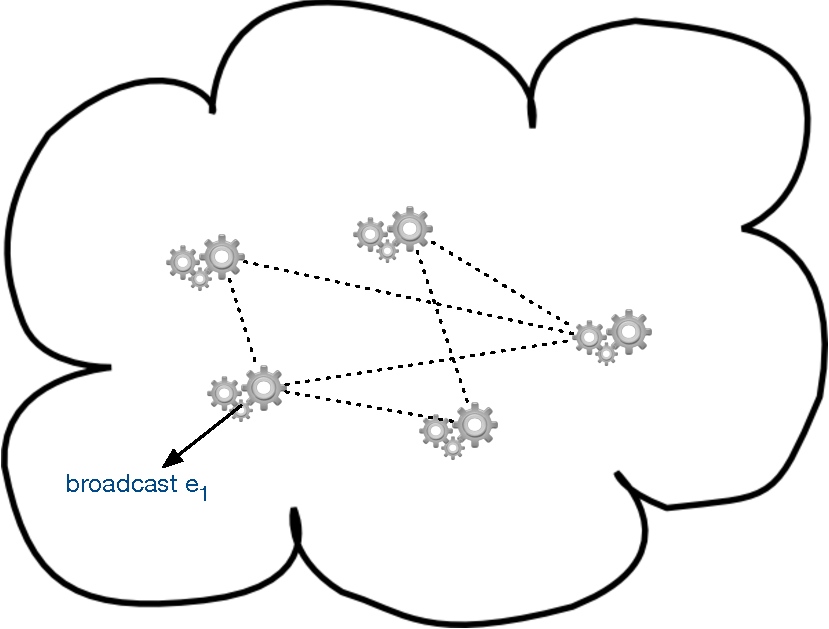
\includegraphics[scale=0.5]{ideab1}
}

\only<3>
{
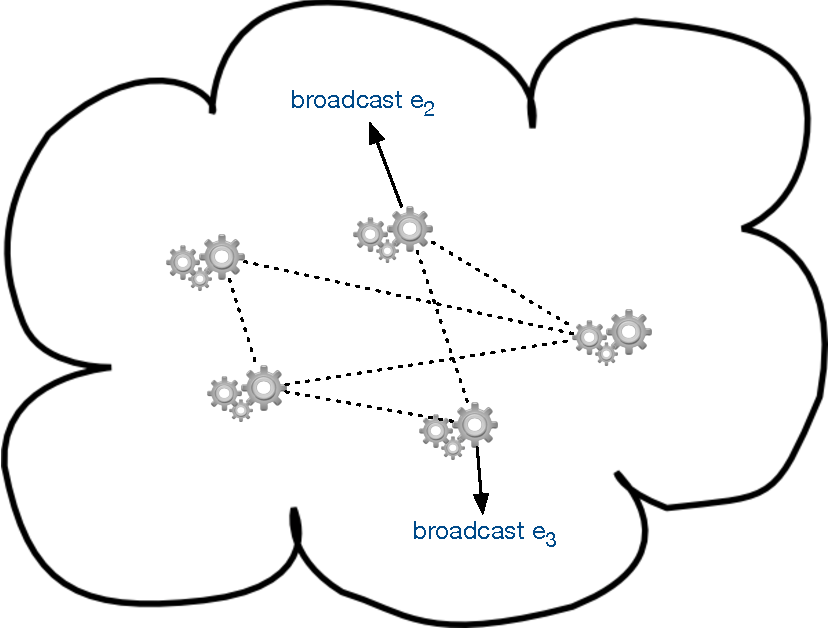
\includegraphics[scale=0.5]{ideab2}
}

\only<4>
{
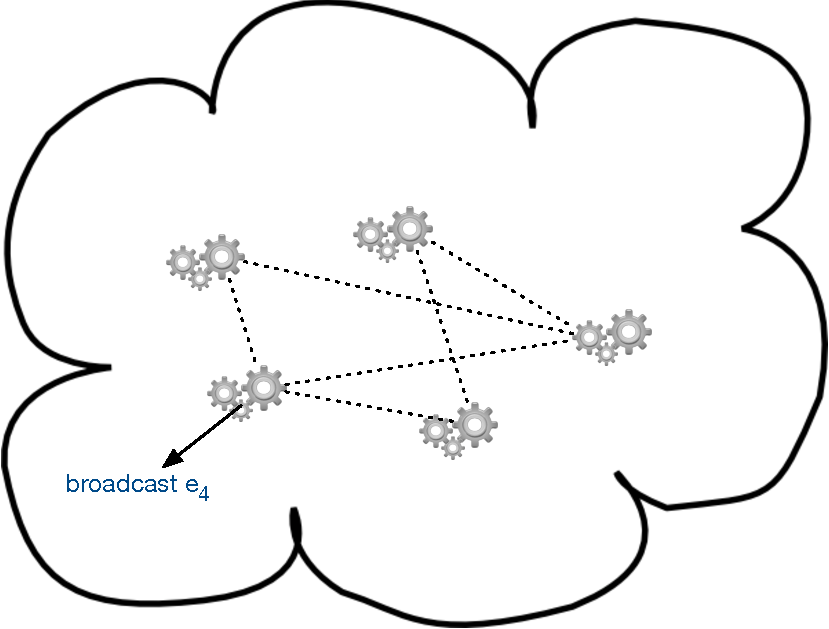
\includegraphics[scale=0.5]{ideab3}
}

\only<5>
{
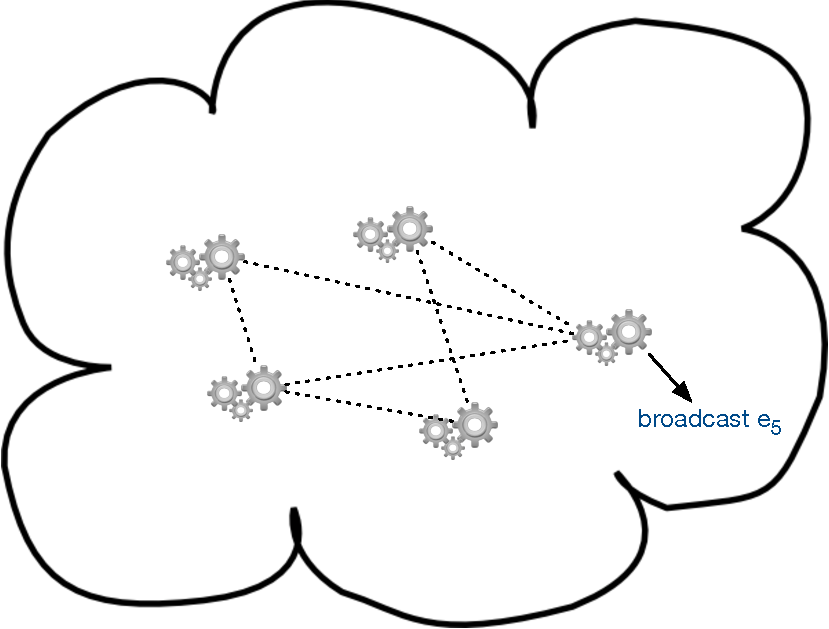
\includegraphics[scale=0.5]{ideab4}
}

\only<6>
{
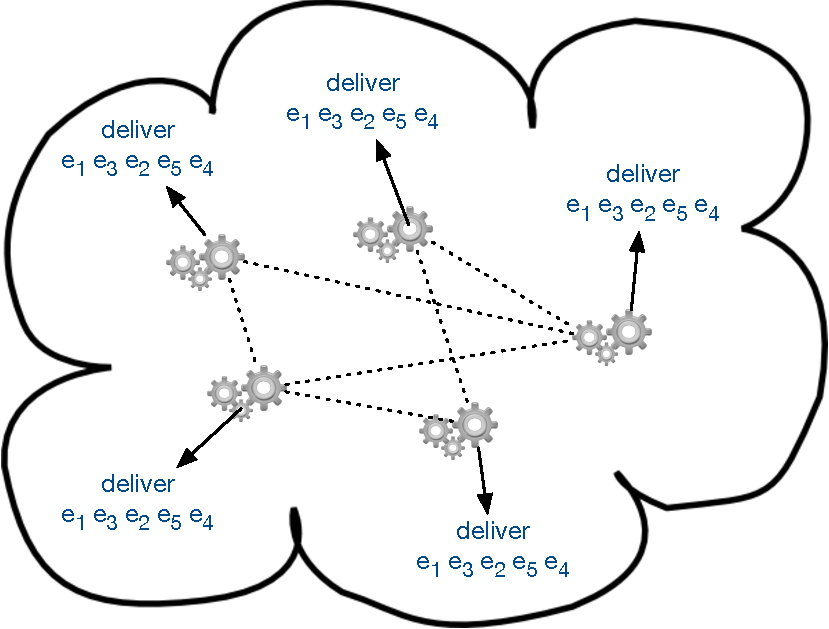
\includegraphics[scale=0.5]{ideadeliver}
}


\end{frame}

% -------------------------------------------------------------------------------

\begin{frame}{... actually, maybe not so simple}
  
  \begin{itemize}

  \item The ordering of events is one of the most fundamental problems in distributed systems.

  \item A large body of research has been dedicated to the design of ordering abstractions with different guarantees and tradeoffs.

\vspace{5mm}

  \begin{snugshade}
            \begin{center}
  In real-life dynamic large-scale settings, deterministic algorithms are prohibitively expensive and/or non-scalable.
   \end{center}
  \end{snugshade}  

 \begin{snugshade}
            \begin{center}
Probabilistic dissemination protocols are highly scalable and resilient to adversarial network conditions, but often overlook stronger properties such as ordering.
   \end{center}
  \end{snugshade}

  %         \begin{snugshade}
  %           \begin{center}
  %     This results in a mismatch between what is expected by distributed applications and the achievable properties in the large-scale systems encountered in the real world.
  %   \end{center}
  % \end{snugshade}
  
\end{itemize}

\end{frame}

% -------------------------------------------------------------------------------

\begin{frame}{State of the art}
  
\begin{itemize}

\item Deterministic total order algorithms [Défago et al. 2004]

\item Optimistic total order algorithms [Pedone \& Schiper 2003]

\item Deterministic algorithms leveraging eventual consistency [Baldoni et al. 2006, Vogels 2009]. 

\item Deterministic algorithms with probabilistic delivery guarantees [Ezhilchelvan 2011] (no ordering properties, not scalable without probabilistic dissemination).

\item Probabilistic algorithms with no or weak ordering guarantees [Birman et al. 1999, Koldehofe 2002, Eugster et al. 2003, Carvalho et al. 2007, ...]

\item Probabilistic total order algorithms assuming static and fully synchronous networks [Hayden \& Birman 1996]

\item $\dots$

  \begin{snugshade}
    To the best of our knowledge, no scalable and robust \\ total order algorithm is available.
  \end{snugshade}

\end{itemize}

\end{frame}

% -------------------------------------------------------------------------------

\subtitle[Properties]{Properties}

% -------------------------------------------------------------------------------

\begin{frame}{Our contribution: \EPTO}
  
  \begin{itemize}

  \item We present and analyze EpTO, a new total order epidemic dissemination algorithm with probabilistic reliability guarantees. 

  \item EpTO guarantees that processes eventually agree on the set of received events with \tc{high probability} and deliver these events in total order to the application. 
  \end{itemize}
  
\end{frame}

% -------------------------------------------------------------------------------

\begin{frame}{Advantages of \EPTO}
  
        EpTO is well-suited for large-scale dynamic distributed systems: 
  \begin{itemize}
 \item Conceptually simple and fully decentralized, not requiring any form of coordination among processes. 

\item Does not require sub-protocols, acknowledgments nor retransmissions.

\item Scalable as the number of events and processes increases.

\item Does not require a global clock nor synchronized processes.

\item Highly robust even when the network suffers from large delays and significant churn and message loss.
\end{itemize}

\end{frame}

% -------------------------------------------------------------------------------

\begin{frame}{\EPTO\ properties}
 
\only<1>
{
\mbox{\ }\vspace{-1mm}
\begin{mdframed}[linecolor=white]

 \hangindent=10pt \textbf{Deterministic Integrity:} 
Every process delivers an event at most once, and only if it was previously broadcast. \medskip
  
\hangindent=10pt \textbf{Deterministic Validity:} Correct processes eventually deliver the events they broadcast. \medskip

  \hangindent=10pt \textbf{Deterministic Total Order:} Process $p$ delivers event $e$ before $e'$ if and only if process $q$ delivers $e$ before $e'$. 
\end{mdframed}

\vspace{5.8mm}

\mbox{\ }\vspace{-2mm}
\begin{mdframed}[linecolor=white]
    \hangindent=10pt \textbf{Probabilistic Agreement:} If a process broadcasts an event~$e$, then with high probability all correct processes eventually deliver it.
  \end{mdframed}
}  


\only<2>
{

Straightforward to prove
\vspace{-2mm}
\begin{mdframed}

 \hangindent=10pt \textbf{Deterministic Integrity:} 
Every process delivers an event at most once, and only if it was previously broadcast. \medskip
  
\hangindent=10pt \textbf{Deterministic Validity:} Correct processes eventually deliver the events they broadcast. \medskip

  \hangindent=10pt \textbf{Deterministic Total Order:} Process $p$ delivers event $e$ before $e'$ if and only if process $q$ delivers $e$ before $e'$. 
\end{mdframed}

\vspace{5.8mm}

\mbox{\ \tc{\ }}
\vspace{-2mm}
 \begin{mdframed}[linecolor=white]
    \hangindent=10pt \textbf{Probabilistic Agreement:} If a process broadcasts an event~$e$, then with high probability all correct processes eventually deliver it.
  \end{mdframed}
}  


\only<3>
{

Straightforward to prove
\vspace{-2mm}
\begin{mdframed}[linecolor=black]

 \hangindent=10pt \textbf{Deterministic Integrity:} 
Every process delivers an event at most once, and only if it was previously broadcast. \medskip
  
\hangindent=10pt \textbf{Deterministic Validity:} Correct processes eventually deliver the events they broadcast. \medskip

   \hangindent=10pt \textbf{Deterministic Total Order:} Process $p$ delivers event $e$ before $e'$ if and only if process $q$ delivers $e$ before $e'$. 
\end{mdframed}

\vspace{5mm}

\tc{More challenging}
\vspace{-2mm}
 \begin{mdframed}[linecolor=blue]
    \hangindent=10pt \textbf{\tc{Probabilistic Agreement}:} If a process broadcasts an event~$e$, then with \tc{high probability} all correct processes eventually deliver it.
  \end{mdframed}
}  

\end{frame}

% -------------------------------------------------------------------------------

\begin{frame}{Probabilistic agreement may create holes \\ in the sequence of delivered events}

  \begin{figure}
    \centering
    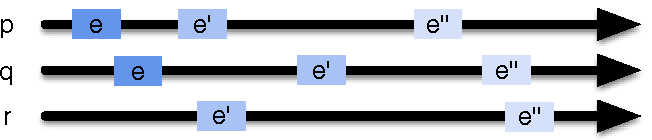
\includegraphics[scale=0.7]{order}
    \caption*{Unlikely but allowed}
  \end{figure}
   

  \begin{figure}
    \centering
    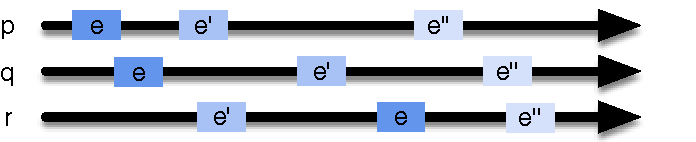
\includegraphics[scale=0.7]{agreement}
    \caption*{Not allowed}
  \end{figure}

\end{frame}

% -------------------------------------------------------------------------------

\subtitle[Balls-into-bins]{Balls-into-bins}

% -------------------------------------------------------------------------------

\begin{frame}{Gossiping with balls and bins}

\only<1>
{  
\vspace{25mm}

\centering
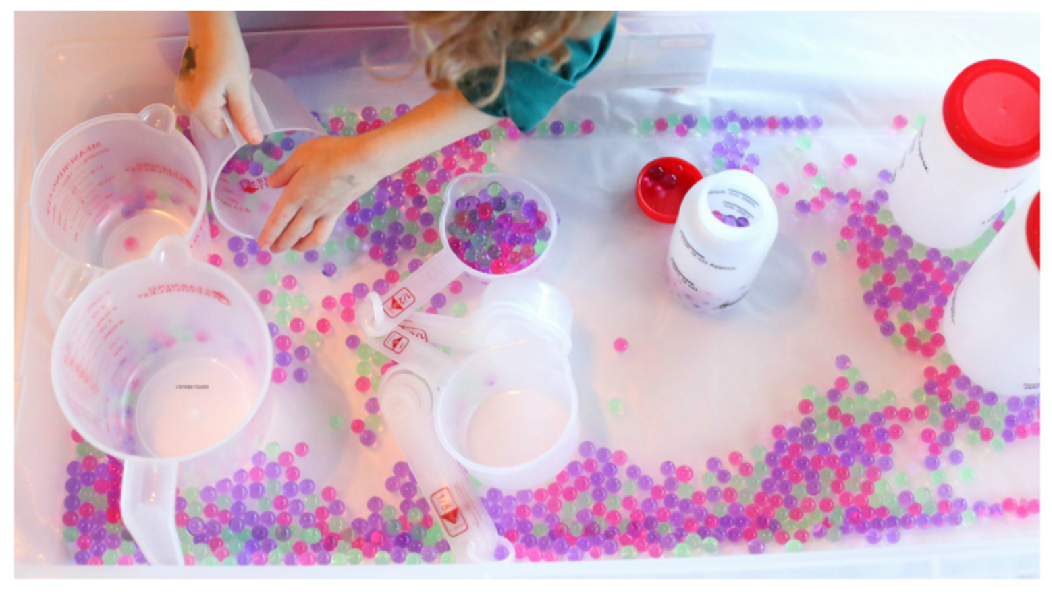
\includegraphics[width=0.9\textwidth]{balls-into-bins}
}

\only<2>
{
\vspace{2.5mm}

\begin{itemize}
  
\item The $n$ processes are abstracted as $n$ bins, and events (rumors) are abstracted as balls.

\end{itemize}

\vspace{4mm}
  
\centering
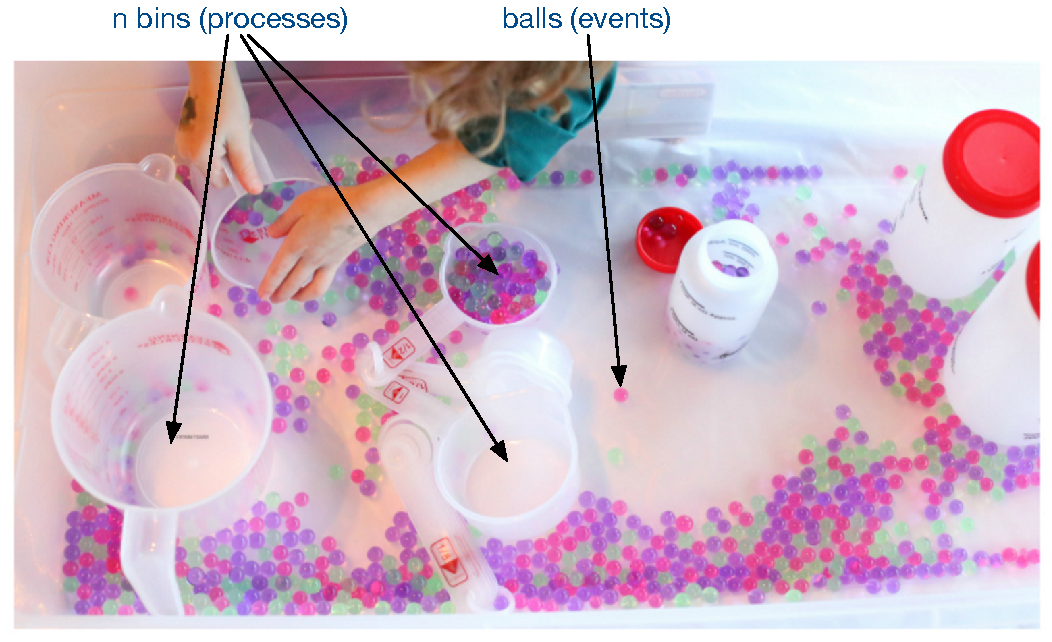
\includegraphics[width=0.9\textwidth]{balls-into-bins-1}
}

\only<3>
{
\vspace{2.5mm}
\begin{itemize}

\item The process starting a rumor sends a ball to $K$ other processes chosen uniformly at random.

\end{itemize}
\vspace{8mm}

\centering
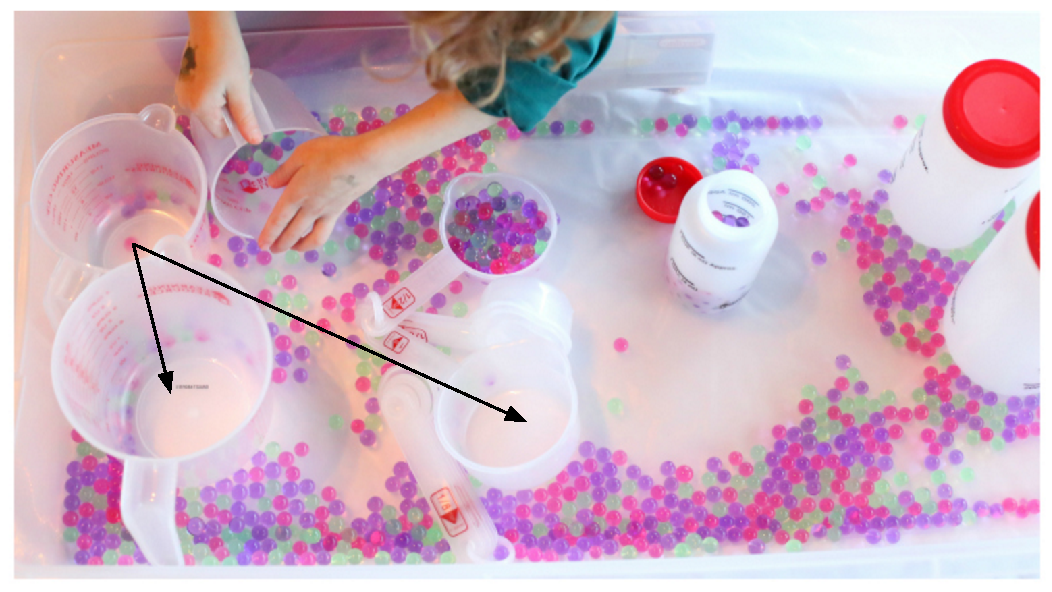
\includegraphics[width=0.9\textwidth]{balls-into-bins-2}

}

 \only<4>
 {
   \begin{itemize}

   \item For each round that follows, the processes which received one or more balls in the previous round a send a ball to K other processes chosen uniformly at random.

\item The protocol terminates after $TTL$ rounds.
   \end{itemize}

 \centering
 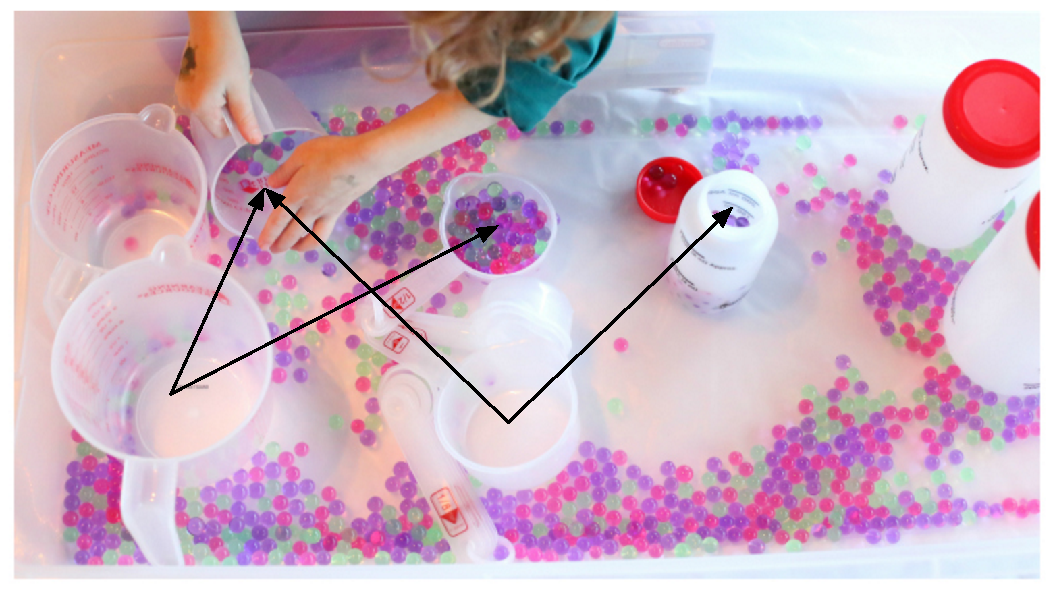
\includegraphics[width=0.9\textwidth]{balls-into-bins-3}
}

\end{frame}

% -------------------------------------------------------------------------------

\begin{frame}{Gossiping with balls and bins}

  \begin{snugshade}    
\begin{theorem}[Koldehofe 2002]
If the gossip protocol uses $K= \lceil \frac{2e \ln n}{\ln \ln n} \rceil$ balls per process and runs for $TTL = (c + 1) \log_2 n$ rounds, where $c > 1$ is a constant, then each process learns the rumor with probability $1 - O\left(n^{-(c+1)}\right)$.  
\end{theorem}
\end{snugshade}


\begin{proof}[Proof idea.]
  \begin{itemize}
  \item During the first $\log_2 n$ rounds, the number of balls disseminated doubles at each round until at least $n$ balls are transmitted per round. 

\item The last $c \log_2 n$ rounds create at least $c n \log_2 n$ balls, which is sufficient to conclude that each process has received at least one ball with high probability.
\end{itemize}
\end{proof}

\end{frame}

% -------------------------------------------------------------------------------

\begin{frame}{The probability of hole can be made orders of magnitude smaller than the probability of a catastrophic hardware or network failure}
  
\begin{figure}
  \centering
  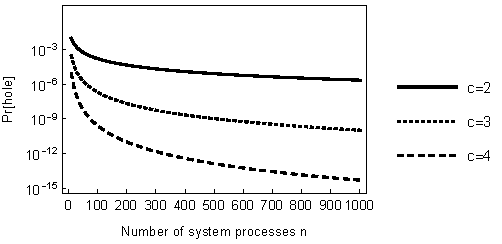
\includegraphics[scale=1.1]{probhole2}
   \caption*{Probability that event $e$ has a hole for at least one process.}
 \end{figure}
 
\end{frame}

% -------------------------------------------------------------------------------

\subtitle[Architecture]{Architecture}

% -------------------------------------------------------------------------------

\begin{frame}{\EPTO \ architecture - dissemination component}


\centering
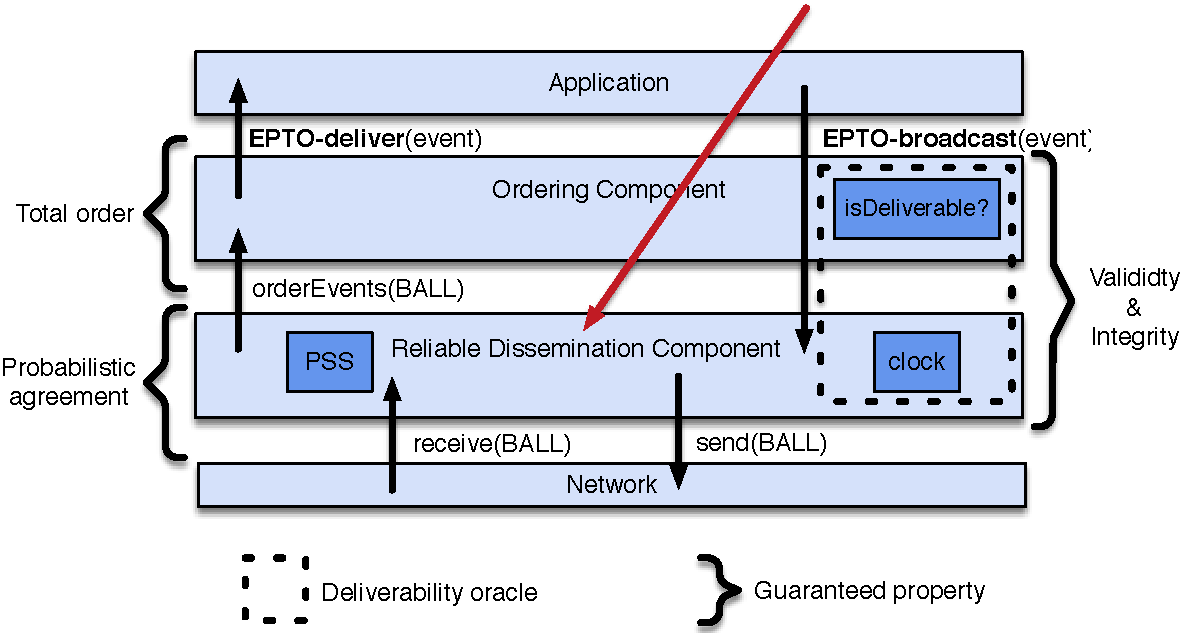
\includegraphics[scale=0.45]{architecture-dissemination}

\vspace{-1mm}

\noindent The dissemination component handles the reception and retransmission of events. 

\begin{itemize}

\item Each event in a ball contains its $id$, $timestamp$, and age~($ttl$).

\item When a ball is received, the age of its events is incremented.

\item At each round, each process groups all the received events in the same ball for the next round.

\end{itemize}

\end{frame}

% -------------------------------------------------------------------------------

\begin{frame}{\EPTO \ architecture - ordering component}

\vspace{-6.5mm}

\centering
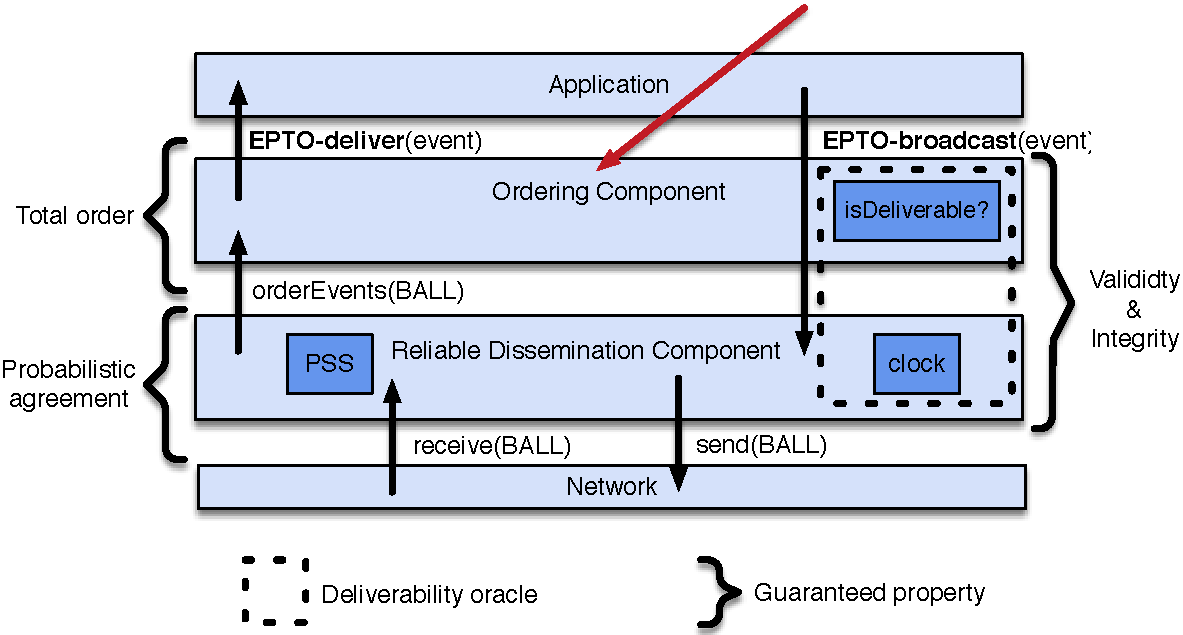
\includegraphics[scale=0.45]{architecture-ordering}
  
The ordering component is responsible of the total order property. 
\begin{itemize}

\item It orders received events based on their timestamp.

\item It ages the received but not yet delivered events.

\item It delivers stable (\tc{old enough}) events to the application.

\end{itemize}

\end{frame}

% -------------------------------------------------------------------------------

\subtitle[Analysis]{Analysis}

% -------------------------------------------------------------------------------

\begin{frame}{Probabilistic agreement property - synchronous \EPTO}

  \begin{snugshade}
    \textbf{Completely unrealistic fairy-tale assumptions:} \\ no churn, access to global time, no lost messages, \\ synchronous rounds and no network latency!!!
  \end{snugshade}

\vspace{-1mm}

\begin{lemma}
\label{lem:globaltime}
If $K \geq \left\lceil\frac{2e\ln n}{\ln\ln n}\right\rceil$ and $TTL \geq \lceil (c+1) \log_2 n \rceil$ where $c>1$, then synchronous \EPTO{} satisfies the Probabilistic Agreement property.
\end{lemma}

\begin{proof}[Proof idea.]
  \begin{itemize}
  \item 
Disseminating events with \EPTO{} corresponds to \emph{aging} them. 

\item When an event $ttl$ reaches $TTL$, a process locally knows that this event has been in the system long enough to reach all other processes with high probability and can be delivered.  

\item Every event is transmitted $\sim c n \log_2 n$ times.
% thus every process receives and delivers every event with high probability.

\end{itemize}

\end{proof}

\end{frame}

% -------------------------------------------------------------------------------

\begin{frame}{\EPTO{} works when all these assumptions are lifted}

  \begin{itemize}

  \item Logical clocks 
\includegraphics[width=5mm]{check}

  \item Process drift  
\includegraphics[width=5mm]{check}

  \item Latency  
\includegraphics[width=5mm]{check}

  \item Churn and message loss 
\includegraphics[width=5mm]{check}

  \end{itemize}

  \begin{snugshade}
    In all cases, we slightly increase the number of rounds and/or the fan-out $K$ and formally prove that every process still receives every event with high probability.
  \end{snugshade}

\end{frame}

% -------------------------------------------------------------------------------

\begin{frame}{Probabilistic agreement property - churn and message loss}
  
\begin{lemma}
\label{lem:churn}
Let $\alpha$ and $\epsilon$ define the churn and message loss rate of the network, and let $K=\left\lceil\frac{2e \ln n}{\ln \ln n} \cdot \frac{n}{n-\alpha}\cdot\frac{1}{1-\epsilon}\right\rceil$. If $TTL \geq \lceil (c+1) \log_2 n \rceil$, then \EPTO{} satisfies the Probabilistic Agreement property.
\end{lemma}

% \begin{proof}

% On average, the number of received balls after churn and lost messages is sufficient.

% \end{proof}

\begin{snugshade}
  EpTO guarantees total ordering and good performance in the presence of significant churn and message loss for large-scale applications.
\end{snugshade}

\end{frame}

% -------------------------------------------------------------------------------

\begin{frame}{Some simulation results}
  
  \begin{snugshade}
In all our experiments, we have not observed a single hole in the sequence of delivered events (I don't count the bugs :-) )
 \end{snugshade}

\begin{figure}[!t]
 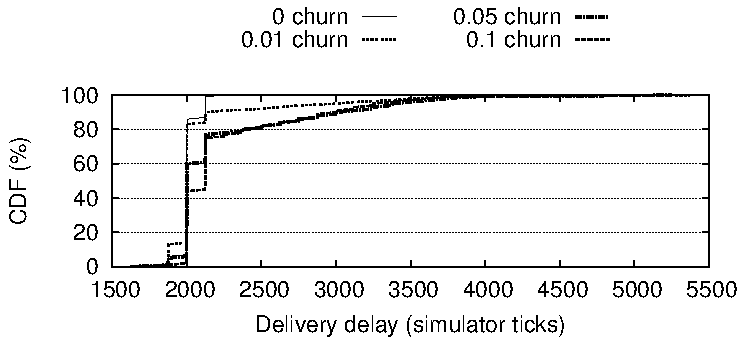
\includegraphics[width=0.5\columnwidth]{deliveryDelay-churn-1} 
  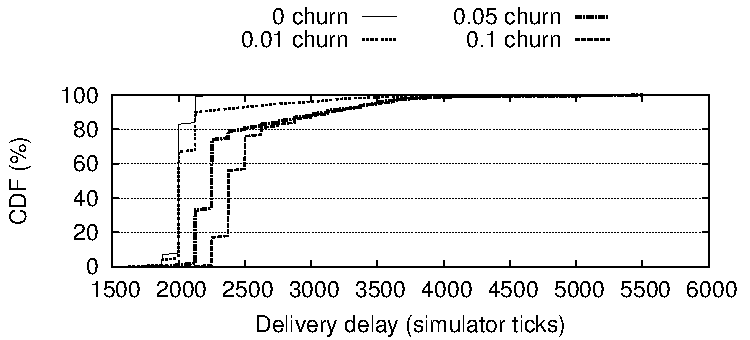
\includegraphics[width=0.5\columnwidth]{deliveryDelay-churn}
\caption{Delivery delay under churn for 500 processes, logical clocks and 5\% broadcast rate. The end-to-end latency distribution drawn from a sample of geographically dispersed PlanetLab nodes. Left figure assumed perfect view, whereas right figure used the Cyclon peer sampling service.}
\label{fig:churn_cyclon}
%\vspace{-3mm}
\end{figure}


\end{frame}

% -------------------------------------------------------------------------------

\subtitle[Conclusion]{Conclusion}

% -------------------------------------------------------------------------------

\begin{frame}{Concluding remarks}

  \begin{itemize}

\item Traditional total order algorithms do not scale well, nor do they work well under challenging network conditions. 

\item EpTO solves both problems at the same time.

\bigskip

\begin{snugshade}

  \begin{itemize}

  \item In the worst case, we can set the algorithm parameters based on the well-behaving nodes (or based on good network conditions) and guarantee that the well-behaving part of the network will satisfy the Probabilistic Agreement property. 

\medskip

\item Bad processes can remain in the network and do not affect the performance of the algorithm. No deterministic algorithm has this property.

  \end{itemize}

\end{snugshade}


  \end{itemize}
  
\end{frame}

% -------------------------------------------------------------------------------

\begin{frame}{Future work}
    
  \begin{itemize}

  \item \emph{In theory there is no difference between theory and practice. But, in practice, there is.} From simulation to real-world implementation.
  
  \item The asymptotics of balls-into-bins problems for probabilistic dissemination can be improved. We found similarities with biometric problems studied in the 1960s estimating the proportion of vectors capable of transmitting viruses in natural populations.

\vspace{-6mm}

  \begin{center}
    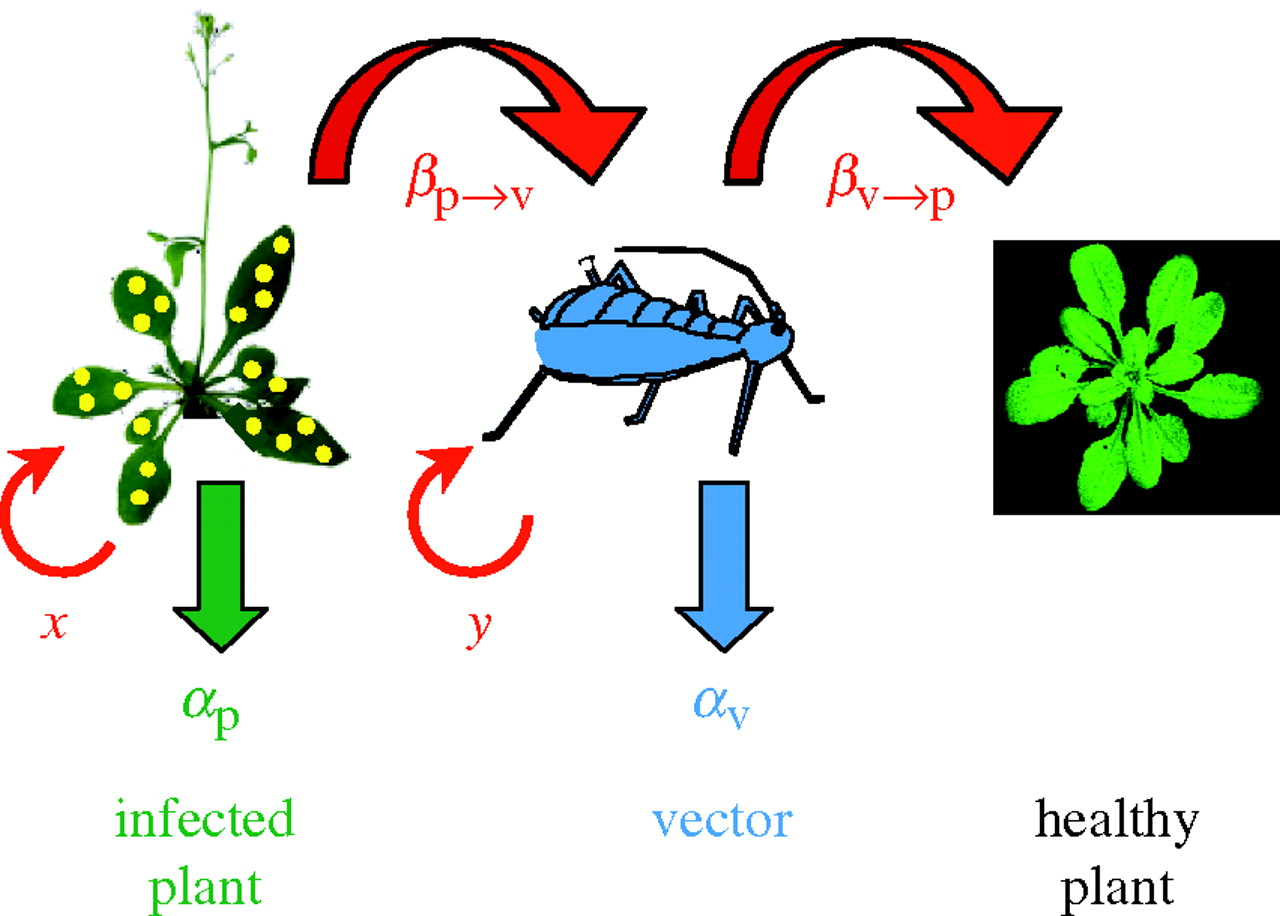
\includegraphics[scale=0.13]{insectes}
  \end{center}

\end{itemize}

\end{frame}

% -------------------------------------------------------------------------------

\begin{frame}[plain]{Thanks for your time. Questions?}
  
  \begin{center}
    
\includegraphics[scale=0.2]{questions}
  \end{center}
  
\end{frame}

% -------------------------------------------------------------------------------

\subtitle[Extra]{Extra}

% -------------------------------------------------------------------------------

\begin{frame}{Probabilistic agreement property - logical time \EPTO}
  
\begin{lemma}
If $K \geq \left\lceil\frac{2e\ln n}{\ln\ln n}\right\rceil$ and $TTL \geq 2 \lceil (c+1) \log_2 n \rceil$ where $c>1$, then \EPTO{} with logical time satisfies the Probabilistic Agreement property.
\end{lemma}

\begin{proof}[Proof idea.]

\centering
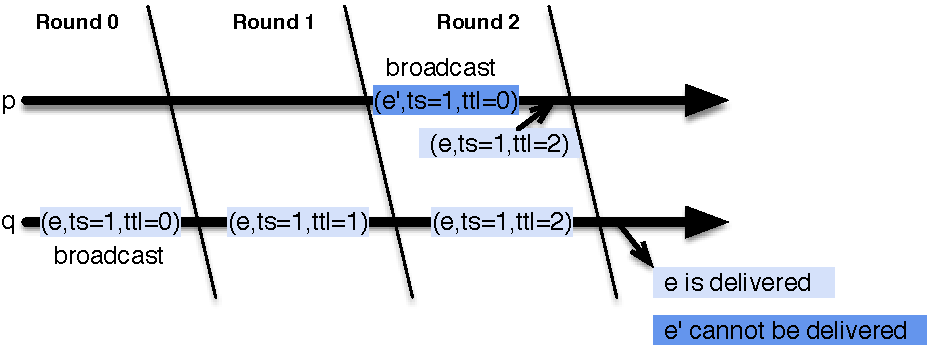
\includegraphics[scale=0.6]{logicalClock}

\end{proof}

\end{frame}

% -------------------------------------------------------------------------------
% -------------------------------------------------------------------------------

\begin{frame}{Probabilistic agreement property - process drift}
  
\begin{lemma}
Let assume that the round duration $\delta$ of each process is always bounded by $\delta_{\min} \leq \delta \leq \delta_{\max}$, that $K \geq \left\lceil\frac{2e\ln n}{\ln\ln n}\right\rceil$, and that $c>1$. If $TTL \geq 2 \lceil (c+1) \log_2 n \rceil \cdot \frac{\delta_{\max}}{\delta_{\min}}$, then \EPTO{} with logical time satisfies the Probabilistic Agreement property.
\end{lemma}

\begin{proof}[Proof idea.]
 The dissemination of an event in the network can be represented as a tree, where the root is the process which broadcasted the event, nodes at depth $d$ for $d \geq 1$ are the processes which are $d$ balls away from the root, and the leaves are the processes that delivered the event. \\ \medskip

The depth of the leaves of the tree are at depth at least $\lceil (c+1) \log_2 n \rceil$.
\end{proof}

\end{frame}

% -------------------------------------------------------------------------------

\begin{frame}{Probabilistic agreement property - network latency}
  
\begin{lemma}
\label{lem:latency}
Let $N_1 \subseteq N$ be a subset of the network such that the latency within $N_1$ is always bounded by $L_\text{max}$. If $\delta > L_{\max}$, then \EPTO{} with logical time satisfies the Probability Agreement property within $N_1$ with $K \geq \left\lceil\frac{2e\ln n}{\ln\ln n}\right\rceil$, $c>1$ and $TTL \geq 2 \lceil (c+1) \log_2 n \rceil+1$. 
\end{lemma}

\begin{proof}[Proof idea.]
Since the latency within $N_1$ is smaller than the round duration, it follows that messages will always reach their destination at most one round after they were transmitted.
\end{proof}

\begin{snugshade}
  \begin{itemize}
  \item By setting the round duration based on the latency of the well-behaving nodes (or on the latency under good network conditions), we can guarantee that the well-behaving part of the network will satisfy the Probabilistic Agreement property. 

\item The processes with large latency can remain in the network and do not slow down the algorithm.

  \end{itemize}

\end{snugshade}

\end{frame}

% -------------------------------------------------------------------------------
% -------------------------------------------------------------------------------

\end{document}

% -------------------------------------------------------------------------------
